\subsection{Latency Profiles and Computational Overhead}
\label{subsec:results_latency}

\subsubsection{Academic Multi-Hop Benchmark (MuSiQue)}
\label{subsubsec:latency_musique}

\begin{table}[htbp]
\centering
\small
\setlength{\tabcolsep}{3.5pt}
\caption{End-to-end execution latency and Time-to-First-Token (TTFT) across 16 pipeline architectures on MuSiQue. Statistical significance flags denote Holm-Bonferroni-adjusted paired Wilcoxon signed-rank tests against the naive baseline.}
\label{tab:latency_musique}
\begin{tabular*}{\linewidth}{@{\extracolsep{\fill}} l r r r r r @{}}
\toprule
\textbf{Pipeline} & \makecell{\textbf{TTFT $P_{50}$}\\\scriptsize{(ms)}} & \makecell{\textbf{TTFT $P_{95}$}\\\scriptsize{(ms)}} & \makecell{\textbf{$T_{\text{total}} P_{50}$}\\\scriptsize{(ms)}} & \makecell{\textbf{$T_{\text{total}} P_{95}$}\\\scriptsize{(ms)}} & \makecell{\textbf{$\Delta T_{\text{total}}$}\\\scriptsize{(\%)}} \\
\midrule
\multicolumn{6}{@{}l@{}}{\textbf{Baseline ($k=0$)}} \\
Naive RAG Baseline & 1990.0 & 3636.0 & 2120.0 & 4173.3 & -- \\
\midrule
\multicolumn{6}{@{}l@{}}{\textbf{Single-Factor Isolated ($k=1$)}} \\
S2B & 1553.0 & 7067.1 & 1684.0 & 7184.9 & -20.6\%\textsuperscript{ns} \\
SR & 1860.5 & 3620.0 & 2035.5 & 3677.1 & -4.0\%\textsuperscript{ns} \\
PC & 1864.0 & 3433.5 & 2020.0 & 3590.3 & -4.7\%\textsuperscript{ns} \\
MC & 2945.0 & 5392.2 & 3060.0 & 5450.8 & +44.3\%\textsuperscript{ns} \\
\midrule
\multicolumn{6}{@{}l@{}}{\textbf{Pairwise Combinations ($k=2$)}} \\
S2B + SR & 1776.5 & 2249.4 & 2018.0 & 2482.1 & -4.8\%\textsuperscript{ns} \\
S2B + PC & 1506.0 & 3087.9 & 1648.0 & 3333.7 & -22.3\%\textsuperscript{ns} \\
S2B + MC & 2722.0 & 3506.5 & 2792.5 & 3565.2 & +31.7\%\textsuperscript{ns} \\
SR + PC & 1716.0 & 3879.6 & 1828.0 & 4026.1 & -13.8\%\textsuperscript{ns} \\
SR + MC & 3111.0 & 3923.0 & 3123.5 & 4051.5 & +47.3\%\textsuperscript{ns} \\
PC + MC & 3593.5 & 6067.5 & 3690.0 & 6123.7 & +74.1\%\textsuperscript{ns} \\
\midrule
\multicolumn{6}{@{}l@{}}{\textbf{Higher-Order Combinations ($k \ge 3$)}} \\
S2B + SR + PC & 1810.5 & 2831.8 & 1897.0 & 2966.0 & -10.5\%\textsuperscript{ns} \\
S2B + SR + MC & 2764.0 & 3599.6 & 2833.5 & 3672.8 & +33.7\%\textsuperscript{ns} \\
S2B + PC + MC & 4975.5 & 12427.9 & 5068.0 & 12531.3 & +139.1\%\textsuperscript{ns} \\
SR + PC + MC & 5619.5 & 20268.6 & 5927.0 & 20432.8 & +179.6\%\textsuperscript{ns} \\
S2B + SR + PC + MC & 4063.0 & 9282.8 & 4177.5 & 9396.1 & +97.1\%\textsuperscript{ns} \\
\bottomrule
\end{tabular*}
\vspace{0.5em}
\parbox{\linewidth}{\footnotesize
\textbf{Notes:} $P_{50}$ and $P_{95}$ denote median and 95th percentile execution latencies. TTFT denotes Time-to-First-Token. $\Delta T_{\text{total}}$ reflects percentage change in median latency relative to the naive baseline. Statistical significance flags denote two-tailed paired Wilcoxon signed-rank tests against the naive baseline with Holm-Bonferroni correction ($^{*} p < 0.05$, $^{**} p < 0.01$, $^{***} p < 0.001$, $\mathrm{ns} = p \ge 0.05$).}
\end{table}


Detailed component-wise execution latency breakdowns decomposing processing duration across dense retrieval, cross-encoder neural re-ranking, prompt caching management, model routing classification, and generative token synthesis are provided in Appendix~\ref{sec:appendix_breakdowns} (Figure~\ref{fig:latency_breakdown_musique}).

\subsubsection{Enterprise Production Corpus}
\label{subsubsec:latency_enterprise}

\begin{table}[htbp]
\centering
\small
\setlength{\tabcolsep}{3.5pt}
\caption{End-to-end execution latency and Time-to-First-Token (TTFT) across 16 pipeline configurations on Enterprise Closed. Statistical significance flags denote Holm-Bonferroni-adjusted paired Wilcoxon signed-rank tests against the naive baseline ($C_0$).}
\label{tab:latency_enterprise}
\begin{tabular*}{\linewidth}{@{\extracolsep{\fill}} l l r r r r r @{}}
\toprule
\textbf{Config} & \textbf{Pipeline} & \makecell{\textbf{TTFT $P_{50}$}\\\scriptsize{(ms)}} & \makecell{\textbf{TTFT $P_{95}$}\\\scriptsize{(ms)}} & \makecell{\textbf{$T_{\text{total}} P_{50}$}\\\scriptsize{(ms)}} & \makecell{\textbf{$T_{\text{total}} P_{95}$}\\\scriptsize{(ms)}} & \makecell{\textbf{$\Delta T_{\text{total}}$}\\\scriptsize{(\%)}} \\
\midrule
\multicolumn{7}{l}{\textbf{Baseline ($k=0$)}} \\
$C_{0}$ & Naive RAG Baseline & 1517.0 & 7878.1 & 1932.5 & 8123.9 & -- \\
\midrule
\multicolumn{7}{l}{\textbf{Single-Factor Isolated ($k=1$)}} \\
$C_{1}$ & S2B & 1486.5 & 19310.8 & 1855.5 & 20167.5 & -4.0\%\textsuperscript{ns} \\
$C_{2}$ & SR & 2128.5 & 20096.0 & 2379.5 & 19946.9 & +23.1\%\textsuperscript{ns} \\
$C_{3}$ & PC & 2596.5 & 13985.9 & 3050.0 & 15803.5 & +57.8\%\textsuperscript{ns} \\
$C_{4}$ & MC & 2002.5 & 10615.3 & 2247.5 & 10511.3 & +16.3\%\textsuperscript{ns} \\
\midrule
\multicolumn{7}{l}{\textbf{Pairwise Combinations ($k=2$)}} \\
$C_{5}$ & S2B + SR & 2935.0 & 37568.9 & 3590.0 & 36934.3 & +85.8\%\textsuperscript{ns} \\
$C_{6}$ & S2B + PC & 1808.5 & 7449.3 & 2113.0 & 7011.8 & +9.3\%\textsuperscript{ns} \\
$C_{7}$ & S2B + MC & 3070.5 & 38226.5 & 3212.0 & 80290.4 & +66.2\%\textsuperscript{ns} \\
$C_{8}$ & SR + PC & 17141.0 & 100664.3 & 17418.0 & 100143.3 & +801.3\%\textsuperscript{ns} \\
$C_{9}$ & SR + MC & 2393.5 & 38900.8 & 2982.5 & 38043.8 & +54.3\%\textsuperscript{ns} \\
$C_{10}$ & PC + MC & 8009.5 & 25023.3 & 8272.5 & 24781.8 & +328.1\%\textsuperscript{ns} \\
\midrule
\multicolumn{7}{l}{\textbf{Higher-Order Triplets \& Full-Stack ($k \ge 3$)}} \\
$C_{11}$ & S2B + SR + PC & 2256.0 & 12359.2 & 2907.5 & 13234.9 & +50.5\%\textsuperscript{ns} \\
$C_{12}$ & S2B + SR + MC & 3115.0 & 31735.2 & 3697.0 & 31503.6 & +91.3\%\textsuperscript{ns} \\
$C_{13}$ & S2B + PC + MC & 6813.5 & 107870.5 & 6797.0 & 107289.1 & +251.7\%\textsuperscript{ns} \\
$C_{14}$ & SR + PC + MC & 4042.0 & 118949.4 & 4050.0 & 118309.8 & +109.6\%\textsuperscript{ns} \\
$C_{15}$ & S2B + SR + PC + MC (Full-Stack) & 8926.0 & 54762.9 & 9346.5 & 54607.5 & +383.6\%\textsuperscript{ns} \\
\bottomrule
\end{tabular*}
\vspace{0.5em}
\parbox{\linewidth}{\footnotesize
\textbf{Notes:} $P_{50}$ and $P_{95}$ denote median and 95th percentile execution latencies. TTFT denotes Time-to-First-Token. $\Delta T_{\text{total}}$ reflects percentage change in median latency relative to baseline ($C_0$). Statistical significance flags denote two-tailed paired Wilcoxon signed-rank tests against baseline ($C_0$) with Holm-Bonferroni correction ($^{*} p < 0.05$, $^{**} p < 0.01$, $^{***} p < 0.001$, $\mathrm{ns} = p \ge 0.05$).}
\end{table}


The corresponding fine-grained phase-wise latency distributions for the enterprise closed corpus are illustrated in Appendix~\ref{sec:appendix_breakdowns} (Figure~\ref{fig:latency_breakdown_enterprise}).

\subsection{Operational Expenditure and Token Dynamics}
\label{subsec:results_cost}

\subsubsection{Academic Multi-Hop Benchmark (MuSiQue)}
\label{subsubsec:cost_musique}

\begin{table}[htbp]
\centering
\small
\setlength{\tabcolsep}{3.5pt}
\caption{Operational cost and token consumption breakdown across 16 pipeline configurations on MuSiQue. Statistical significance flags denote Holm-Bonferroni-adjusted paired Wilcoxon signed-rank tests against the naive baseline ($C_0$).}
\label{tab:cost_musique}
\begin{tabular*}{\linewidth}{@{\extracolsep{\fill}} l l r r r r r @{}}
\toprule
\textbf{Config} & \textbf{Pipeline} & \makecell{\textbf{Uncached}\\\textbf{Prompt Tok}} & \makecell{\textbf{Cached}\\\textbf{Prompt Tok}} & \makecell{\textbf{Output}\\\textbf{Tokens}} & \makecell{\textbf{Cost / 1k}\\\scriptsize{(\$)}} & \makecell{\textbf{$\Delta$ Cost}\\\scriptsize{(\%)}} \\
\midrule
\multicolumn{7}{l}{\textbf{Baseline ($k=0$)}} \\
$C_{0}$ & Naive RAG Baseline & 7,436 & 408 & 23 & \$1.191 & -- \\
\midrule
\multicolumn{7}{l}{\textbf{Single-Factor Isolated ($k=1$)}} \\
$C_{1}$ & S2B & 6,710 & 1,224 & 29 & \$1.208 & +1.4\%\textsuperscript{ns} \\
$C_{2}$ & SR & 4,903 & 3,059 & 25 & \$6.210 & +421.5\%\textsuperscript{*} \\
$C_{3}$ & PC & 689 & 7,153 & 26 & \$0.495 & -58.5\%\textsuperscript{*} \\
$C_{4}$ & MC & 7,173 & 680 & 19 & \$7.060 & +493.0\%\textsuperscript{*} \\
\midrule
\multicolumn{7}{l}{\textbf{Pairwise Combinations ($k=2$)}} \\
$C_{5}$ & S2B + SR & 6,793 & 1,224 & 31 & \$6.221 & +422.5\%\textsuperscript{*} \\
$C_{6}$ & S2B + PC & 778 & 7,153 & 30 & \$0.511 & -57.1\%\textsuperscript{*} \\
$C_{7}$ & S2B + MC & 6,710 & 1,224 & 22 & \$6.574 & +452.1\%\textsuperscript{*} \\
$C_{8}$ & SR + PC & 808 & 7,153 & 28 & \$5.514 & +363.1\%\textsuperscript{*} \\
$C_{9}$ & SR + MC & 7,962 & 0 & 20 & \$11.544 & +869.5\%\textsuperscript{*} \\
$C_{10}$ & PC + MC & 689 & 7,153 & 25 & \$3.157 & +165.1\%\textsuperscript{ns} \\
\midrule
\multicolumn{7}{l}{\textbf{Higher-Order Triplets \& Full-Stack ($k \ge 3$)}} \\
$C_{11}$ & S2B + SR + PC & 862 & 7,153 & 32 & \$5.524 & +364.0\%\textsuperscript{*} \\
$C_{12}$ & S2B + SR + MC & 6,793 & 1,224 & 18 & \$11.514 & +867.0\%\textsuperscript{*} \\
$C_{13}$ & S2B + PC + MC & 778 & 7,153 & 20 & \$3.233 & +171.5\%\textsuperscript{ns} \\
$C_{14}$ & SR + PC + MC & 808 & 7,153 & 24 & \$8.498 & +613.7\%\textsuperscript{*} \\
$C_{15}$ & S2B + SR + PC + MC (Full-Stack) & 862 & 7,153 & 21 & \$8.181 & +587.1\%\textsuperscript{*} \\
\bottomrule
\end{tabular*}
\vspace{0.5em}
\parbox{\linewidth}{\footnotesize
\textbf{Notes:} Prompt and completion tokens represent query sample averages. If cached prompt tokens are reported ($N_{\text{cached}} > 0$), uncached prompt tokens are computed as $\max(0, N_{\text{prompt}} - N_{\text{cached}})$. Cost reflects Google Cloud Gemini Enterprise platform pricing normalized per 1,000 queries. $\Delta\text{Cost}$ reflects percentage change relative to baseline ($C_0$). Statistical significance flags denote two-tailed paired Wilcoxon signed-rank tests against baseline ($C_0$) with Holm-Bonferroni correction ($^{*} p < 0.05$, $^{**} p < 0.01$, $^{***} p < 0.001$, $\mathrm{ns} = p \ge 0.05$).}
\end{table}


Detailed phase-wise monetary cost decompositions across uncached prompt prefill, context cache lookups, generative completion tokens, auxiliary re-ranking services, and router classifications are provided in Appendix~\ref{sec:appendix_breakdowns} (Figure~\ref{fig:cost_breakdown_musique}).

\subsubsection{Enterprise Production Corpus}
\label{subsubsec:cost_enterprise}

\begin{table}[htbp]
\centering
\small
\setlength{\tabcolsep}{3.5pt}
\caption{Operational cost and token consumption breakdown across 16 pipeline configurations on Enterprise Closed. Statistical significance flags denote Holm-Bonferroni-adjusted paired Wilcoxon signed-rank tests against the naive baseline ($C_0$).}
\label{tab:cost_enterprise}
\begin{tabular*}{\linewidth}{@{\extracolsep{\fill}} l l r r r r r @{}}
\toprule
\textbf{Config} & \textbf{Pipeline} & \makecell{\textbf{Uncached}\\\textbf{Prompt Tok}} & \makecell{\textbf{Cached}\\\textbf{Prompt Tok}} & \makecell{\textbf{Output}\\\textbf{Tokens}} & \makecell{\textbf{Cost / 1k}\\\scriptsize{(\$)}} & \makecell{\textbf{$\Delta$ Cost}\\\scriptsize{(\%)}} \\
\midrule
\multicolumn{7}{l}{\textbf{Baseline ($k=0$)}} \\
$C_{0}$ & Naive RAG Baseline & 4,036 & 4,488 & 100 & \$1.339 & -- \\
\midrule
\multicolumn{7}{l}{\textbf{Single-Factor Isolated ($k=1$)}} \\
$C_{1}$ & S2B & 8,728 & 612 & 105 & \$1.464 & +9.4\%\textsuperscript{ns} \\
$C_{2}$ & SR & 6,941 & 1,836 & 82 & \$6.366 & +375.4\%\textsuperscript{*} \\
$C_{3}$ & PC & 1,369 & 7,153 & 99 & \$0.640 & -52.2\%\textsuperscript{*} \\
$C_{4}$ & MC & 6,484 & 2,040 & 79 & \$1.081 & -19.3\%\textsuperscript{ns} \\
\midrule
\multicolumn{7}{l}{\textbf{Pairwise Combinations ($k=2$)}} \\
$C_{5}$ & S2B + SR & 7,241 & 1,837 & 121 & \$6.435 & +380.6\%\textsuperscript{*} \\
$C_{6}$ & S2B + PC & 2,185 & 7,153 & 100 & \$0.763 & -43.0\%\textsuperscript{ns} \\
$C_{7}$ & S2B + MC & 7,879 & 612 & 58 & \$2.014 & +50.4\%\textsuperscript{ns} \\
$C_{8}$ & SR + PC & 1,622 & 7,153 & 93 & \$5.782 & +331.8\%\textsuperscript{*} \\
$C_{9}$ & SR + MC & 8,165 & 612 & 59 & \$7.017 & +424.0\%\textsuperscript{*} \\
$C_{10}$ & PC + MC & 1,369 & 7,153 & 76 & \$1.901 & +42.0\%\textsuperscript{ns} \\
\midrule
\multicolumn{7}{l}{\textbf{Higher-Order Triplets \& Full-Stack ($k \ge 3$)}} \\
$C_{11}$ & S2B + SR + PC & 1,922 & 7,153 & 84 & \$5.714 & +326.8\%\textsuperscript{*} \\
$C_{12}$ & S2B + SR + MC & 7,445 & 1,632 & 75 & \$7.178 & +436.1\%\textsuperscript{*} \\
$C_{13}$ & S2B + PC + MC & 1,865 & 7,153 & 66 & \$0.654 & -51.2\%\textsuperscript{ns} \\
$C_{14}$ & SR + PC + MC & 1,625 & 7,153 & 62 & \$7.099 & +430.1\%\textsuperscript{*} \\
$C_{15}$ & S2B + SR + PC + MC (Full-Stack) & 1,922 & 7,153 & 81 & \$5.789 & +332.4\%\textsuperscript{*} \\
\bottomrule
\end{tabular*}
\vspace{0.5em}
\parbox{\linewidth}{\footnotesize
\textbf{Notes:} Prompt and completion tokens represent query sample averages. If cached prompt tokens are reported ($N_{\text{cached}} > 0$), uncached prompt tokens are computed as $\max(0, N_{\text{prompt}} - N_{\text{cached}})$. Cost reflects Google Cloud Gemini Enterprise platform pricing normalized per 1,000 queries. $\Delta\text{Cost}$ reflects percentage change relative to baseline ($C_0$). Statistical significance flags denote two-tailed paired Wilcoxon signed-rank tests against baseline ($C_0$) with Holm-Bonferroni correction ($^{*} p < 0.05$, $^{**} p < 0.01$, $^{***} p < 0.001$, $\mathrm{ns} = p \ge 0.05$).}
\end{table}


The corresponding component-wise operational expenditure breakdown per 1,000 queries for the enterprise closed corpus is illustrated in Appendix~\ref{sec:appendix_breakdowns} (Figure~\ref{fig:cost_breakdown_enterprise}).

\subsection{Retrieval and Generation Quality}
\label{subsec:results_quality}

\subsubsection{Academic Multi-Hop Benchmark (MuSiQue)}
\label{subsubsec:quality_musique}

\begin{table}[htbp]
\centering
\scriptsize
\setlength{\tabcolsep}{2.2pt}
\caption{Retrieval, generation, and multi-hop reasoning quality metrics across 16 pipeline configurations on the MuSiQue benchmark ($N = 10$). Statistical significance flags denote Holm-Bonferroni-adjusted paired Wilcoxon signed-rank tests against the naive baseline ($C_0$).}
\label{tab:quality_musique}
\begin{tabular*}{\linewidth}{@{\extracolsep{\fill}} l l c c c c c c c @{}}
\toprule
\textbf{Config} & \textbf{Pipeline} & \makecell{\textbf{Context}\\\textbf{Precision}} & \makecell{\textbf{Context}\\\textbf{Recall}} & \makecell{\textbf{Faithful-}\\\textbf{ness}} & \makecell{\textbf{Answer}\\\textbf{Relevancy}} & \makecell{\textbf{Token}\\\textbf{F1 (\%)}} & \makecell{\textbf{Exact}\\\textbf{Match (\%)}} & \makecell{\textbf{Composite}\\\textbf{Quality $Q$}} \\
\midrule
\multicolumn{9}{l}{\textbf{Baseline ($k=0$)}} \\
$C_{0}$ & Naive RAG Baseline & 0.400 & 0.800 & 0.733 & 0.612 & 41.5\% & 20.0\% & 0.3334 \\
\midrule
\multicolumn{9}{l}{\textbf{Single-Factor Isolated ($k=1$)}} \\
$C_{1}$ & S2B & 0.433 & 0.800 & 0.950 & 0.569 & 33.1\% & 10.0\% & \textbf{0.4431}\textsuperscript{ns} \\
$C_{2}$ & SR & 0.450 & 0.750 & 0.850 & 0.612 & 36.7\% & 10.0\% & 0.3942\textsuperscript{ns} \\
$C_{3}$ & PC & 0.450 & 0.833 & 0.683 & 0.601 & 41.3\% & 20.0\% & 0.3847\textsuperscript{ns} \\
$C_{4}$ & MC & 0.500 & 0.889 & 0.537 & 0.369 & 28.5\% & 11.1\% & 0.3406\textsuperscript{ns} \\
\midrule
\multicolumn{9}{l}{\textbf{Pairwise Combinations ($k=2$)}} \\
$C_{5}$ & S2B + SR & 0.550 & 0.900 & 0.777 & 0.503 & 32.0\% & 10.0\% & 0.3791\textsuperscript{ns} \\
$C_{6}$ & S2B + PC & 0.383 & 0.625 & 0.900 & 0.559 & 36.1\% & 10.0\% & 0.3014\textsuperscript{ns} \\
$C_{7}$ & S2B + MC & 0.483 & 0.850 & 0.700 & 0.556 & 32.8\% & 10.0\% & 0.2756\textsuperscript{ns} \\
$C_{8}$ & SR + PC & 0.450 & 0.900 & 0.900 & 0.638 & 36.6\% & 10.0\% & 0.4054\textsuperscript{ns} \\
$C_{9}$ & SR + MC & 0.350 & 0.850 & 0.500 & 0.431 & 27.6\% & 10.0\% & 0.3238\textsuperscript{ns} \\
$C_{10}$ & PC + MC & 0.383 & 1.000 & 0.650 & 0.460 & 28.3\% & 10.0\% & 0.3683\textsuperscript{ns} \\
\midrule
\multicolumn{9}{l}{\textbf{Higher-Order Triplets \& Full-Stack ($k \ge 3$)}} \\
$C_{11}$ & S2B + SR + PC & 0.450 & 0.500 & 0.783 & 0.552 & 37.5\% & 20.0\% & 0.3801\textsuperscript{ns} \\
$C_{12}$ & S2B + SR + MC & 0.550 & 0.550 & 0.625 & 0.462 & 24.6\% & 10.0\% & 0.3809\textsuperscript{ns} \\
$C_{13}$ & S2B + PC + MC & 0.483 & 0.800 & 0.683 & 0.452 & 36.7\% & 20.0\% & 0.3594\textsuperscript{ns} \\
$C_{14}$ & SR + PC + MC & 0.350 & 0.767 & 0.700 & 0.430 & 20.4\% & 0.0\% & 0.2430\textsuperscript{ns} \\
$C_{15}$ & S2B + SR + PC + MC (Full-Stack) & 0.450 & 0.817 & 0.750 & 0.430 & 26.1\% & 10.0\% & 0.3122\textsuperscript{ns} \\
\bottomrule
\end{tabular*}
\vspace{0.5em}
\parbox{\linewidth}{\footnotesize
\textbf{Notes:} Context Precision, Context Recall, Faithfulness, and Answer Relevancy are evaluated via RAGAS~\citep{es2024ragas} exclusively on answerable queries. Token F1 and Exact Match evaluate lexical overlap against reference answers. Composite Quality $Q \in [0, 1]$ represents the regularized harmonic mean across the four RAGAS dimensions (Equation~\ref{eq:composite_quality}, $\epsilon = 10^{-4}$). Highest composite quality score is highlighted in bold. Statistical significance flags denote two-tailed paired Wilcoxon signed-rank tests against baseline ($C_0$) with Holm-Bonferroni correction ($^{*} p < 0.05$, $^{**} p < 0.01$, $^{***} p < 0.001$, $\mathrm{ns} = p \ge 0.05$).}
\end{table}


Configuration-level multi-dimensional response quality profiles spanning Context Precision, Context Recall, Faithfulness, and Answer Relevancy across architectural tiers are visualized as tier-stratified lollipop plots in Appendix~\ref{sec:appendix_breakdowns} (Figure~\ref{fig:quality_lollipop_musique}).

\subsubsection{Enterprise Production Corpus}
\label{subsubsec:quality_enterprise}

\begin{table}[htbp]
\centering
\scriptsize
\setlength{\tabcolsep}{2.2pt}
\caption{Retrieval, generation, and out-of-domain rejection quality metrics across 16 pipeline architectures on the Enterprise Knowledge Corpus ($N = 10$). Statistical significance flags denote Holm-Bonferroni-adjusted paired Wilcoxon signed-rank tests against the naive baseline.}
\label{tab:quality_enterprise}
\begin{tabular*}{\linewidth}{@{\extracolsep{\fill}} l c c c c c c @{}}
\toprule
\textbf{Pipeline} & \makecell{\textbf{Context}\\\textbf{Precision}} & \makecell{\textbf{Context}\\\textbf{Recall}} & \makecell{\textbf{Faithful-}\\\textbf{ness}} & \makecell{\textbf{Answer}\\\textbf{Relevancy}} & \makecell{\textbf{Refusal Acc. /}\\\textbf{FRR (\%)}} & \makecell{\textbf{Composite}\\\textbf{Quality $Q$}} \\
\midrule
\multicolumn{7}{@{}l@{}}{\textbf{Baseline ($k=0$)}} \\
Naive RAG Baseline & 0.818 & 1.000 & 0.808 & 0.747 & 100.0\% / 12.5\% & 0.7314 \\
\midrule
\multicolumn{7}{@{}l@{}}{\textbf{Single-Factor Isolated ($k=1$)}} \\
S2B & 0.765 & 0.938 & 0.734 & 0.547 & 100.0\% / 37.5\% & 0.5710\textsuperscript{ns} \\
SR & 0.829 & 1.000 & 0.625 & 0.726 & 100.0\% / 25.0\% & 0.6113\textsuperscript{ns} \\
PC & 0.808 & 0.938 & 0.729 & 0.555 & 100.0\% / 25.0\% & 0.6099\textsuperscript{ns} \\
MC & 0.808 & 0.938 & 0.975 & 0.772 & 100.0\% / 0.0\% & \textbf{0.8522}\textsuperscript{ns} \\
\midrule
\multicolumn{7}{@{}l@{}}{\textbf{Pairwise Combinations ($k=2$)}} \\
S2B + SR & 0.733 & 0.875 & 0.768 & 0.656 & 100.0\% / 12.5\% & 0.6735\textsuperscript{ns} \\
S2B + PC & 0.880 & 0.938 & 0.784 & 0.670 & 100.0\% / 12.5\% & 0.7456\textsuperscript{ns} \\
S2B + MC & 0.755 & 0.938 & 0.625 & 0.637 & 100.0\% / 37.5\% & 0.5803\textsuperscript{ns} \\
SR + PC & 0.801 & 0.875 & 0.750 & 0.574 & 100.0\% / 25.0\% & 0.6512\textsuperscript{ns} \\
SR + MC & 0.751 & 0.750 & 0.625 & 0.485 & 100.0\% / 37.5\% & 0.3265\textsuperscript{ns} \\
PC + MC & 0.731 & 1.000 & 0.938 & 0.791 & 100.0\% / 0.0\% & 0.7474\textsuperscript{ns} \\
\midrule
\multicolumn{7}{@{}l@{}}{\textbf{Higher-Order Combinations ($k \ge 3$)}} \\
S2B + SR + PC & 0.754 & 0.875 & 0.812 & 0.643 & 100.0\% / 12.5\% & 0.6777\textsuperscript{ns} \\
S2B + SR + MC & 0.744 & 0.875 & 0.720 & 0.555 & 100.0\% / 25.0\% & 0.4461\textsuperscript{ns} \\
S2B + PC + MC & 0.763 & 1.000 & 0.638 & 0.543 & 100.0\% / 28.6\% & 0.5638\textsuperscript{ns} \\
SR + PC + MC & 0.796 & 1.000 & 0.571 & 0.444 & 100.0\% / 42.9\% & 0.4927\textsuperscript{ns} \\
S2B + SR + PC + MC & 0.802 & 0.875 & 0.875 & 0.660 & 100.0\% / 12.5\% & 0.7129\textsuperscript{ns} \\
\bottomrule
\end{tabular*}
\vspace{0.5em}
\parbox{\linewidth}{\footnotesize
\textbf{Notes:} Context Precision, Context Recall, Faithfulness, and Answer Relevancy are evaluated via RAGAS~\citep{es2024ragas} exclusively on answerable queries. Refusal Accuracy evaluates correct abstention on unanswerable out-of-domain (OOD) queries, while False Refusal Rate (FRR) measures erroneous abstention on answerable queries. Composite Quality $Q \in [0, 1]$ represents the regularized harmonic mean across the four RAGAS dimensions on answerable queries (Equation~\ref{eq:composite_quality}, $\epsilon = 10^{-4}$). Statistical significance flags denote two-tailed paired Wilcoxon signed-rank tests against the naive baseline with Holm-Bonferroni correction ($^{*} p < 0.05$, $^{**} p < 0.01$, $^{***} p < 0.001$, $\mathrm{ns} = p \ge 0.05$).}
\end{table}


The corresponding four-dimensional quality metric distributions for the enterprise closed benchmark corpus are depicted in Appendix~\ref{sec:appendix_breakdowns} (Figure~\ref{fig:quality_lollipop_enterprise}).

\subsection{Trade-off Equilibrium and Pareto Frontier}
\label{subsec:results_pareto}

\subsubsection{Academic Multi-Hop Benchmark (MuSiQue)}
\label{subsubsec:pareto_musique}

\begin{table}[htbp]
\centering
\small
\setlength{\tabcolsep}{3.5pt}
\caption{Multi-objective Pareto efficiency and 3D non-domination trade-off metrics across 16 pipeline architectures on MuSiQue.}
\label{tab:pareto_musique}
\begin{tabular*}{\linewidth}{@{\extracolsep{\fill}} l c r r r r c @{}}
\toprule
\textbf{Pipeline} & \makecell{\textbf{Composite}\\\textbf{Quality $Q$}} & \makecell{\textbf{Cost / 1k}\\\scriptsize{(\$)}} & \makecell{\textbf{$T_{\text{total}} P_{50}$}\\\scriptsize{(s)}} & \textbf{QPD} & \textbf{QPS} & \makecell{\textbf{Pareto}\\\textbf{Optimal}} \\
\midrule
\multicolumn{7}{@{}l@{}}{\textbf{Baseline ($k=0$)}} \\
Naive RAG Baseline & 0.6747 & \$11.972 & 2.12 & 56 & 0.32 & No \\
\midrule
\multicolumn{7}{@{}l@{}}{\textbf{Single-Factor Isolated ($k=1$)}} \\
S2B & 0.6735 & \$12.161 & 1.68 & 55 & 0.40 & \textbf{Yes} \\
SR & 0.6626 & \$17.169 & 2.04 & 39 & 0.33 & No \\
PC & 0.6772 & \$3.411 & 2.02 & 199 & 0.34 & \textbf{Yes} \\
MC & 0.3987 & \$14.672 & 3.06 & 27 & 0.13 & No \\
\midrule
\multicolumn{7}{@{}l@{}}{\textbf{Pairwise Combinations ($k=2$)}} \\
S2B + SR & 0.7029 & \$17.302 & 2.02 & 41 & 0.35 & \textbf{Yes} \\
S2B + PC & 0.6688 & \$3.586 & 1.65 & 187 & 0.41 & \textbf{Yes} \\
S2B + MC & 0.5353 & \$14.589 & 2.79 & 37 & 0.19 & No \\
SR + PC & 0.7004 & \$8.613 & 1.83 & 81 & 0.38 & \textbf{Yes} \\
SR + MC & 0.4844 & \$19.603 & 3.12 & 25 & 0.16 & No \\
PC + MC & 0.5309 & \$5.373 & 3.69 & 99 & 0.14 & No \\
\midrule
\multicolumn{7}{@{}l@{}}{\textbf{Higher-Order Combinations ($k \ge 3$)}} \\
S2B + SR + PC & 0.6837 & \$8.727 & 1.90 & 78 & 0.36 & No \\
S2B + SR + MC & 0.4661 & \$19.644 & 2.83 & 24 & 0.16 & No \\
S2B + PC + MC & 0.4805 & \$5.492 & 5.07 & 87 & 0.09 & No \\
SR + PC + MC & 0.4855 & \$10.639 & 5.93 & 46 & 0.08 & No \\
S2B + SR + PC + MC & 0.4752 & \$10.593 & 4.18 & 45 & 0.11 & No \\
\bottomrule
\end{tabular*}
\vspace{0.5em}
\parbox{\linewidth}{\footnotesize
\textbf{Notes:} Composite Quality $Q \in [0, 1]$ represents the regularized harmonic mean across RAGAS dimensions (Equation~\ref{eq:composite_quality}, $\epsilon = 10^{-4}$). Cost reflects Google Cloud Gemini Enterprise platform pricing normalized per 1,000 queries. $T_{\text{total}} P_{50}$ represents median execution latency in seconds. Quality per Dollar ($\mathrm{QPD} = Q / \text{Cost}$) and Quality per Second ($\mathrm{QPS} = Q / T_{\text{total}}$) measure resource efficiency. Pareto optimality denotes non-domination in the 3D trade-off space $(\max Q, \min \text{Cost}, \min T_{\text{total}})$.}
\end{table}


\begin{figure}[!htbp]
\centering
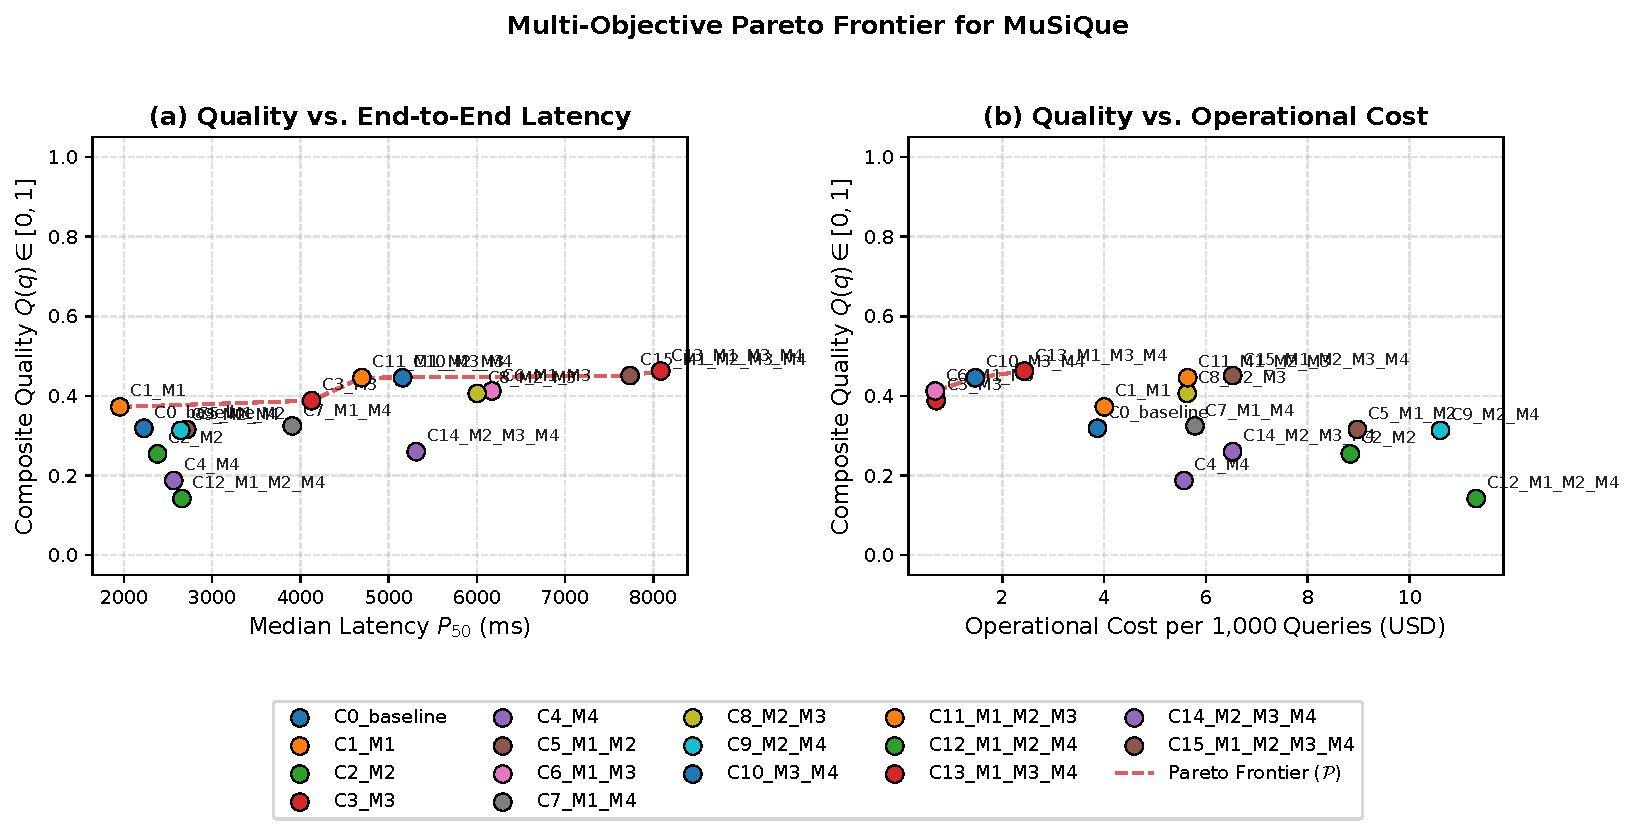
\includegraphics[width=\linewidth]{figures/musique/pareto_frontier_musique.pdf}
\caption{Empirical Pareto frontier of Composite Quality ($Q$) versus median end-to-end execution latency ($T_{\text{total}}\ P_{50}$) and operational expenditure ($\text{Cost}_{1\text{k}}$) on the academic multi-hop benchmark (MuSiQue). Solid lines delineate the non-dominated empirical Pareto frontier across configurations.}
\label{fig:pareto_frontier_musique}
\end{figure}

\subsubsection{Enterprise Production Corpus}
\label{subsubsec:pareto_enterprise}

\begin{table}[htbp]
\centering
\small
\setlength{\tabcolsep}{3.5pt}
\caption{Multi-objective Pareto efficiency and 3D non-domination trade-off metrics across 16 pipeline configurations on Enterprise Closed.}
\label{tab:pareto_enterprise}
\begin{tabular*}{\linewidth}{@{\extracolsep{\fill}} l l c r r r r c @{}}
\toprule
\textbf{Config} & \textbf{Pipeline} & \makecell{\textbf{Composite}\\\textbf{Quality $Q$}} & \makecell{\textbf{Cost / 1k}\\\scriptsize{(\$)}} & \makecell{\textbf{$T_{\text{total}} P_{50}$}\\\scriptsize{(s)}} & \textbf{QPD} & \textbf{QPS} & \makecell{\textbf{Pareto}\\\textbf{Optimal}} \\
\midrule
\multicolumn{8}{l}{\textbf{Baseline ($k=0$)}} \\
$C_{0}$ & Naive RAG Baseline & 0.7314 & \$1.339 & 1.93 & 546 & 0.23 & \textbf{Yes} \\
\midrule
\multicolumn{8}{l}{\textbf{Single-Factor Isolated ($k=1$)}} \\
$C_{1}$ & S2B & 0.5710 & \$1.464 & 1.86 & 390 & 0.11 & \textbf{Yes} \\
$C_{2}$ & SR & 0.6113 & \$6.366 & 2.38 & 96 & 0.11 & No \\
$C_{3}$ & PC & 0.6099 & \$0.640 & 3.05 & 953 & 0.12 & \textbf{Yes} \\
$C_{4}$ & MC & 0.8522 & \$1.081 & 2.25 & 788 & 0.22 & \textbf{Yes} \\
\midrule
\multicolumn{8}{l}{\textbf{Pairwise Combinations ($k=2$)}} \\
$C_{5}$ & S2B + SR & 0.6735 & \$6.435 & 3.59 & 105 & 0.06 & No \\
$C_{6}$ & S2B + PC & 0.7456 & \$0.763 & 2.11 & 977 & 0.24 & \textbf{Yes} \\
$C_{7}$ & S2B + MC & 0.5803 & \$2.014 & 3.21 & 288 & 0.03 & No \\
$C_{8}$ & SR + PC & 0.6512 & \$5.782 & 17.42 & 113 & 0.02 & No \\
$C_{9}$ & SR + MC & 0.3265 & \$7.017 & 2.98 & 47 & 0.03 & No \\
$C_{10}$ & PC + MC & 0.7474 & \$1.901 & 8.27 & 393 & 0.07 & No \\
\midrule
\multicolumn{8}{l}{\textbf{Higher-Order Triplets \& Full-Stack ($k \ge 3$)}} \\
$C_{11}$ & S2B + SR + PC & 0.6777 & \$5.714 & 2.91 & 119 & 0.12 & No \\
$C_{12}$ & S2B + SR + MC & 0.4461 & \$7.178 & 3.70 & 62 & 0.05 & No \\
$C_{13}$ & S2B + PC + MC & 0.5638 & \$0.654 & 6.80 & 862 & 0.02 & No \\
$C_{14}$ & SR + PC + MC & 0.4927 & \$7.099 & 4.05 & 69 & 0.01 & No \\
$C_{15}$ & S2B + SR + PC + MC (Full-Stack) & 0.7129 & \$5.789 & 9.35 & 123 & 0.04 & No \\
\bottomrule
\end{tabular*}
\vspace{0.5em}
\parbox{\linewidth}{\footnotesize
\textbf{Notes:} Composite Quality $Q \in [0, 1]$ represents the regularized harmonic mean across RAGAS dimensions (Equation~\ref{eq:composite_quality}, $\epsilon = 10^{-4}$). Cost reflects Google Cloud Gemini Enterprise platform pricing normalized per 1,000 queries. $T_{\text{total}} P_{50}$ represents median execution latency in seconds. Quality per Dollar ($\mathrm{QPD} = Q / \text{Cost}$) and Quality per Second ($\mathrm{QPS} = Q / T_{\text{total}}$) measure resource efficiency. Pareto optimality denotes non-domination in the 3D trade-off space $(\max Q, \min \text{Cost}, \min T_{\text{total}})$.}
\end{table}


\begin{figure}[!htbp]
\centering
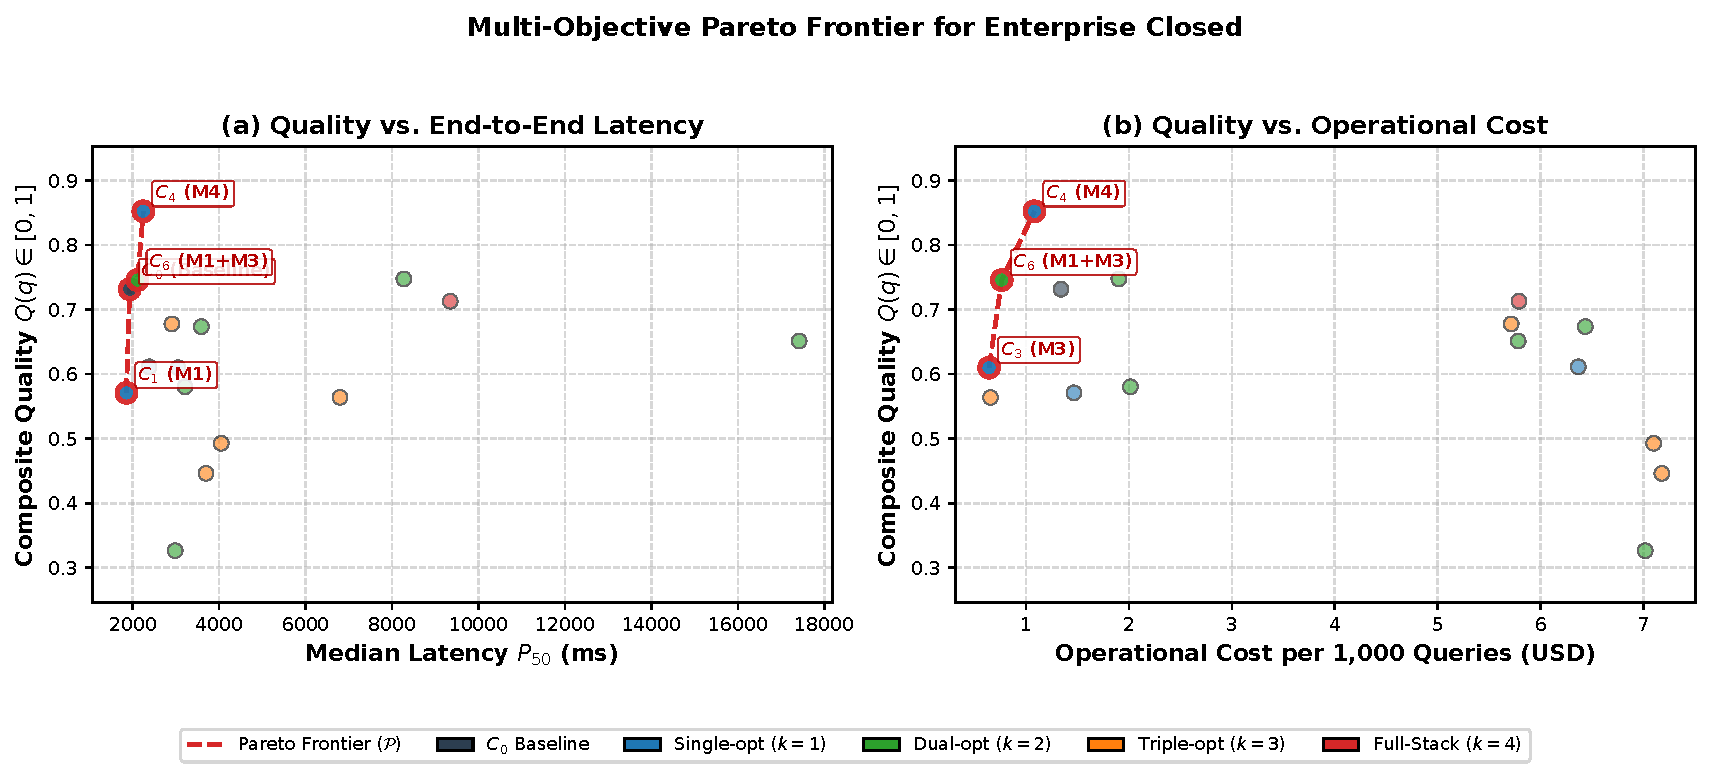
\includegraphics[width=\linewidth]{figures/enterprise_closed/pareto_frontier_enterprise_closed.pdf}
\caption{Empirical Pareto frontier of Composite Quality ($Q$) versus median end-to-end execution latency ($T_{\text{total}}\ P_{50}$) and operational expenditure ($\text{Cost}_{1\text{k}}$) on the enterprise closed benchmark corpus. Solid lines delineate the non-dominated empirical Pareto frontier across configurations.}
\label{fig:pareto_frontier_enterprise}
\end{figure}

\subsection{Executive Performance Delta Synthesis}
\label{subsec:results_delta_heatmap}

To provide a consolidated cross-dimensional view of all 15 architectural optimization treatments relative to the unoptimized naive baseline, Figure~\ref{fig:quality_delta_matrix_musique} and Figure~\ref{fig:quality_delta_matrix_enterprise} visualize relative percentage improvements (green) and regressions (red) across all four RAGAS quality dimensions, Composite Quality ($Q$), median end-to-end latency ($P_{50}$), and operational expenditure per 1,000 queries.

\begin{figure}[!htbp]
\centering
\begin{subfigure}{\linewidth}
  \centering
  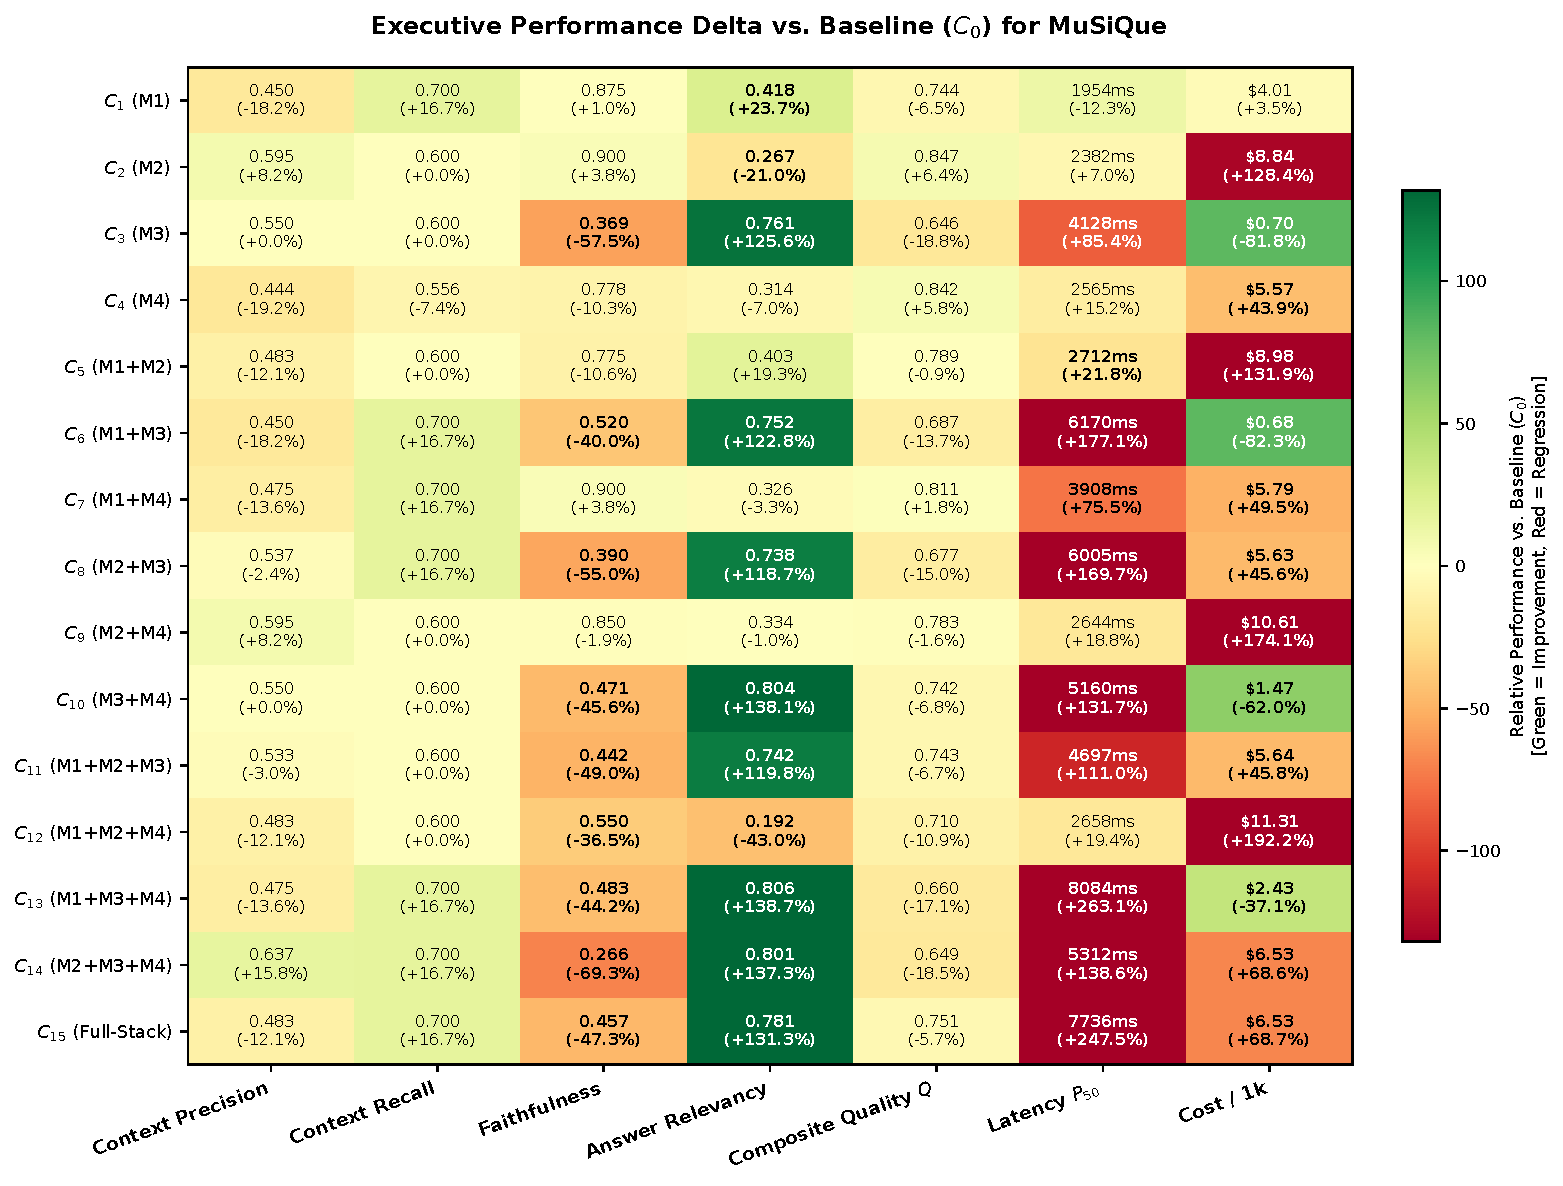
\includegraphics[width=0.78\linewidth]{figures/musique/quality_delta_matrix_musique.pdf}
  \caption{Academic multi-hop benchmark (MuSiQue)}
  \label{fig:quality_delta_matrix_musique}
\end{subfigure}
\\[1ex]
\begin{subfigure}{\linewidth}
  \centering
  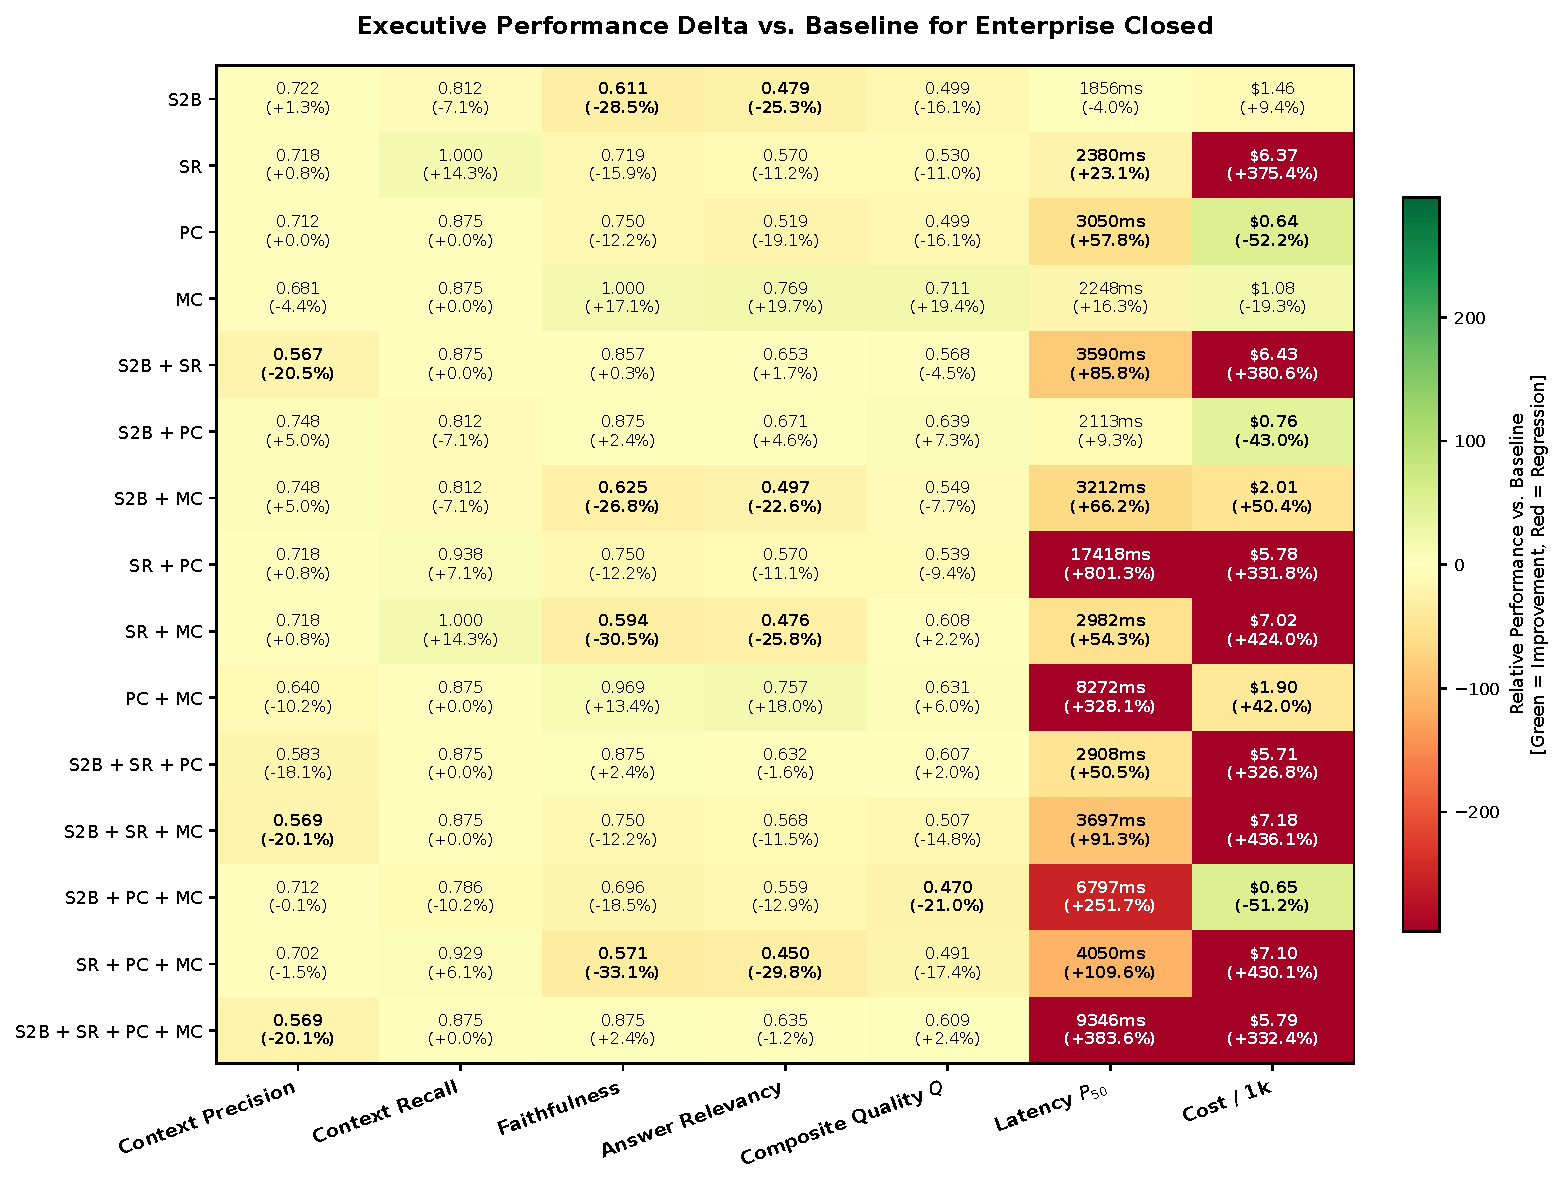
\includegraphics[width=0.78\linewidth]{figures/enterprise_closed/quality_delta_matrix_enterprise_closed.pdf}
  \caption{Enterprise closed benchmark corpus}
  \label{fig:quality_delta_matrix_enterprise}
\end{subfigure}
\caption{Executive performance delta heatmaps relative to the naive baseline on (a) MuSiQue and (b) Enterprise Closed. Cells display absolute metrics alongside relative percentage changes ($\pm\%$). Diverging color gradient highlights performance improvements (green) versus cost/latency regressions (red).}
\label{fig:quality_delta_matrix_combined}
\end{figure}
